% 1998 上海文科第20题：抛物线、焦点D、点E及过D的割线关系示意；不按比例、不编码题设未给的精确斜率。
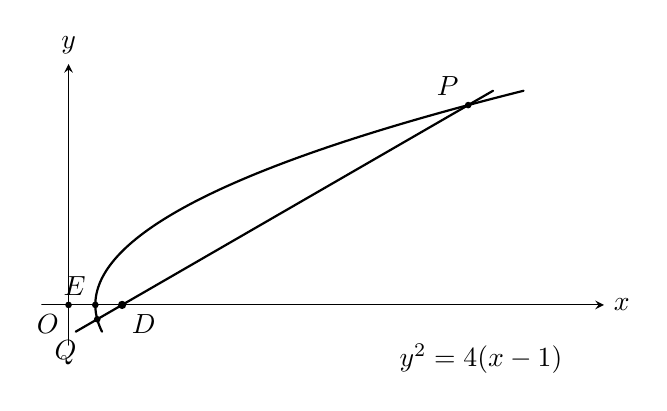
\begin{tikzpicture}[x=0.34cm,y=0.34cm,>=stealth,line cap=round,line join=round]
  \draw[->] (-1,0)--(20,0) node[right] {$x$};
  \draw[->] (0,-1.5)--(0,9) node[above] {$y$};
  \draw[thick,domain=-1:8,samples=100] plot ({1+\x*\x/4},{\x});
  % 示出一条过焦点D的示意割线(斜率1/sqrt(3))；非源卷坐标，不按比例。
  \draw[thick,domain=-1:8,variable=\y] plot ({2+sqrt(3)*\y},{\y});
  \coordinate (P) at ({2+sqrt(3)*(2*sqrt(3)+4)},{2*sqrt(3)+4});
  \coordinate (Q) at ({2+sqrt(3)*(2*sqrt(3)-4)},{2*sqrt(3)-4});
  \fill (0,0) circle (1.2pt) node[below left] {$O$};
  \fill (1,0) circle (1.2pt) node[above left] {$E$};
  \fill (2,0) circle (1.5pt) node[below right] {$D$};
  \fill (P) circle (1.2pt) node[above left] {$P$};
  \fill (Q) circle (1.2pt) node[below left=4pt] {$Q$};
  \node[below right] at (12,-1.1) {$y^2=4(x-1)$};
\end{tikzpicture}
